\subsubsection{Iteration 4: Downgraded White-Box Playground}

\paragraph{Redesign}

In the previous iteration, performance limitations of the target device were identified as a critical constraint. To address this issue, the realistic city environment was removed. The redesigned environment retains only essential elements, including collision boundaries and a predefined flight route, to support the goal-directed navigation.

\paragraph{Enactment}

As illustrated in \cref{fig:white-box}, the player operates the quadcopter within a simplified white-box environment. This environment consists of minimal visual features, focusing on spatial structure and navigational constraints rather than visual realism.

\begin{figure}[H]
\caption{Player controlling the quadcopter in a white-box playground}
\label{fig:white-box}
\centering
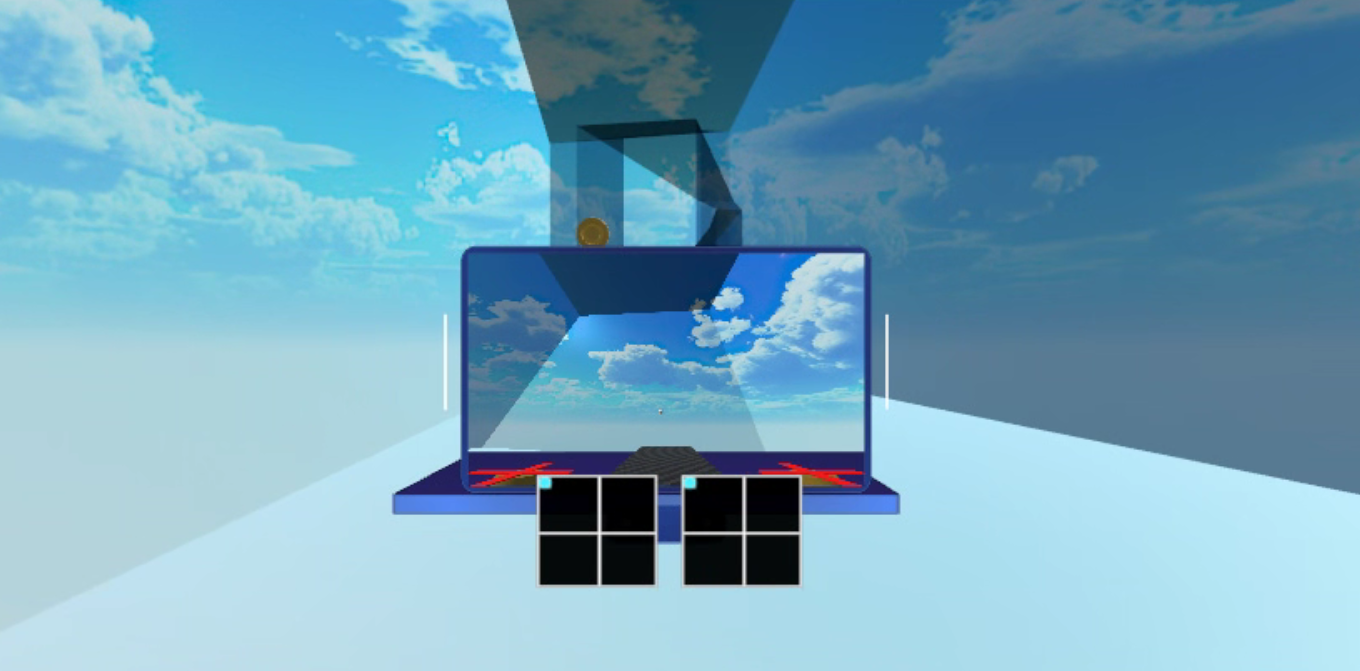
\includegraphics[width=0.8\linewidth]{img/white-box.png}
\end{figure}

\paragraph{Analysis}

The simplified environment is expected to improve system performance and provide a more stable interaction experience. However, user testing has not yet been conducted due to time constraints. Future evaluation is required to assess its effectiveness.

% TODO: Need test play, only 3 days left!!!!
